% Author: Izaak Neutelings (Februari 2021)
\documentclass[border=3pt,tikz]{standalone}
\usepackage{amsmath} % for \dfrac
\usepackage{physics,siunitx}
\usepackage{tikz,pgfplots}
\usepackage[outline]{contour} % glow around text
\contourlength{1.0pt}
\usetikzlibrary{angles,quotes} % for pic (angle labels)
\usetikzlibrary{arrows.meta}
\usetikzlibrary{decorations.markings}
\tikzset{>=latex} % for LaTeX arrow head
\usepackage{xcolor}

\colorlet{xcol}{blue!60!black}
\colorlet{myred}{red!85!black}
\colorlet{myblue}{blue!80!black}
\colorlet{mycyan}{cyan!80!black}
\colorlet{mygreen}{green!70!black}
\colorlet{myorange}{orange!90!black!80}
\colorlet{mypurple}{red!50!blue!90!black!80}
\colorlet{mydarkred}{myred!80!black}
\colorlet{mydarkblue}{myblue!80!black}
\tikzstyle{xline}=[xcol,thick]
\tikzstyle{Tline}=[line width=0.6]
\tikzstyle{width}=[{Latex[length=5,width=3]}-{Latex[length=5,width=3]},thick]
\def\tick#1#2{\draw[thick] (#1)++(#2:0.12) --++ (#2-180:0.24)}
\def\N{100} % number of samples


\begin{document}


% HARMONIC OSCILLATOR FORCE
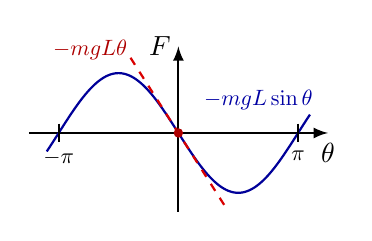
\begin{tikzpicture}
  \message{^^JHarmonic oscillation}
  \def\ymax{1.0}  % max y axis
  \def\xmax{1.9}  % max x axis
  \def\A{0.76}        % amplitude
  \def\T{(1.6*\xmax)} % period
  \draw[->,thick] (0,-\ymax) -- (0,1.1*\ymax) node[left=-1] {$F$};
  \draw[->,thick] (-\xmax,0) -- (\xmax,0) node[below] {$\theta$};
  \draw[xline,samples=100+\N,smooth,variable=\x,domain=-0.88*\xmax:0.88*\xmax]
    plot(\x,{-\A*sin(360/\T*\x)});
  \draw[xline,myred,dashed,samples=\N,smooth,variable=\x,domain=-0.20*\T:0.20*\T] %,line cap=round
    plot(\x,{-\A*2*pi/\T*\x});
  \fill[myred!80!black] (0,0) circle(0.06);
  \tick{{-\T/2},0}{90} node[below=0,scale=0.8] {$-\pi$};
  \tick{{ \T/2},0}{90} node[below=0,scale=0.8] {$\pi$};
  \node[mydarkblue,above left=0,scale=0.8] at (0.95*\xmax,0.25*\A) {$-mgL\sin\theta$};
  \node[mydarkred,above left=0,scale=0.8] at (-0.29*\xmax,1.1*\A) {$-mgL\theta$};
\end{tikzpicture}


% HARMONIC OSCILLATOR ENERGY
\def\ymax{1.4} % max y axis
\begin{tikzpicture}
  \def\xmax{2.6} % max x axis
  \message{^^JHarmonic oscillation}
  \def\A{0.6}         % amplitude
  \def\T{(0.7*\xmax)} % period
  \draw[->,thick] (0,-0.2*\ymax) -- (0,1.1*\ymax) node[left=-1] {$U$};
  \draw[->,thick] (-\xmax,0) -- (\xmax,0) node[below] {$\theta$};
  \draw[xline,samples=100+\N,smooth,variable=\x,domain=-0.94*\xmax:0.94*\xmax]
    plot(\x,{\A-\A*cos(360/\T*\x)});
  \draw[xline,myred,dashed,samples=\N,smooth,variable=\x,domain={-0.33*\T}:{0.34*\T}]
    plot(\x,{\A/2*(2*pi*\x/\T)^2});
  \fill[myred!80!black] (0,0) circle(0.06);
  \tick{{\T},0}{90} node[below=0,scale=0.8] {$2\pi$};
  \tick{{-\T},0}{90} node[below=0,scale=0.8] {$-2\pi$};
  \node[mydarkred,above left,scale=0.8] at ({-0.28*\T},2.05*\A) {$\frac{mgL}{2}\theta^2$};
  \node[mydarkblue,above right,scale=0.8] at ({0.43*\T},1.95*\A) {$mgL(1-\cos\theta)$}; %U(\theta)=
\end{tikzpicture}


% MORSE POTENTIAL
\begin{tikzpicture}
  \message{^^JMorse potential}
  \def\xmax{3.2} % max x axis
  \def\A{1}
  \def\b{2.3}
  \def\a{(0.26*\xmax)}
  \draw[->,thick] (0,-0.2*\ymax) -- (0,1.1*\ymax) node[left=-1] {$U$};
  \draw[->,thick] (-0.2*\ymax,0) -- (\xmax,0) node[below] {$r$};
  \draw[xline,samples=100+\N,smooth,variable=\x,domain=0.15*\xmax:0.94*\xmax]
    plot(\x,{\A*(1-exp(-\b*(\x-\a)))^2});
  \draw[xline,myred,dashed,samples=\N,smooth,variable=\x,domain=0.44*\a:1.55*\a] %,line cap=round
    plot(\x,{\A*\b^2*(\x-\a)^2});
  \fill[myred!80!black] ({\a},0) circle(0.06);
  \tick{{\a},0}{90} node[below=0,scale=0.8] {$r_0$};
  \node[mydarkblue,above right,scale=0.8] at (0.45*\xmax,0.2*\A) {$D\left(1-e^{-a(r-r_0)}\right)^2$};
  \node[mydarkred,scale=0.8] at (0.51*\xmax,0.89*\ymax) {$Da^2(r-r_0)^2$};
\end{tikzpicture}


\end{document}
